\documentclass[runningheads,a4paper]{llncs}

\usepackage[T1]{fontenc}
\usepackage[utf8]{inputenc}
\usepackage{lmodern}
\usepackage{graphicx}
\usepackage{amsmath}
\usepackage{amssymb}
\usepackage{booktabs}
\usepackage{array}
\usepackage{url}
\usepackage{xcolor}
\definecolor{wfBlueFill}{RGB}{232,242,255}
\definecolor{wfBlueDraw}{RGB}{43,101,169}
\definecolor{wfTealFill}{RGB}{225,246,242}
\definecolor{wfTealDraw}{RGB}{30,132,118}
\definecolor{wfAmberFill}{RGB}{255,242,218}
\definecolor{wfAmberDraw}{RGB}{176,112,22}
\definecolor{wfVioletFill}{RGB}{242,235,255}
\definecolor{wfVioletDraw}{RGB}{111,82,170}
\definecolor{wfGreenFill}{RGB}{232,247,231}
\definecolor{wfGreenDraw}{RGB}{73,136,63}
\usepackage[hypertexnames=false]{hyperref}
\hypersetup{
  hidelinks,
  pdfborder={0 0 0}
}
\usepackage{placeins}
\usepackage{algorithm}
\usepackage{algorithmic}
\usepackage{tikz}
\usetikzlibrary{arrows.meta,positioning}

\setlength{\textfloatsep}{7pt plus 2pt minus 2pt}
\setlength{\floatsep}{6pt plus 2pt minus 2pt}
\setlength{\intextsep}{6pt plus 2pt minus 2pt}
\setlength{\abovecaptionskip}{3pt}
\setlength{\belowcaptionskip}{0pt}
\emergencystretch=1.5em

\begin{document}

\title{No-PWM Power Estimation for Fixed-Wing UAVs: Rolling Validation and Energy Audit Support}

\titlerunning{No-PWM UAV Power Estimation}

\author{Nhat Truong\inst{1} \and Thu Le\inst{1,2,3} \and Hoang Duc Tai\inst{1}}

\authorrunning{N. Truong et al.}

\institute{FPT University, Ho Chi Minh City, Vietnam \and
Faculty of Information Technology, University of Science, Ho Chi Minh City, Vietnam \and
Vietnam National University, Ho Chi Minh City, Vietnam\\
\email{truong16102006@gmail.com, thulvm@fpt.edu.vn, ductaiph810@gmail.com}}

\maketitle

\begin{abstract}
Fixed-wing UAV fleet managers need reliable power estimates for charging plans, mission review, and energy anomaly screening. PWM, voltage, current, and actuator channels are predictive, but they may be unavailable or too close to the target for a leakage-audited benchmark. This study evaluates No-PWM power estimation from state-time telemetry on a cleaned IDF-DS Holybro/Pixhawk subset with 118 flights, 60,454 rows, and 33 columns. Under chronological rolling validation, the VIF-safe GRU selected after development-only Pearson/VIF pruning achieves aggregate C4--C7 RMSLE 0.2514, RMSE 20.92\,W, MAE 15.16\,W, and $R^2=0.8927$. C4--C6 remain stable, while C7 exposes distribution shift. Held-out predictions are also aggregated into flight-level energy indicators, watch-list evidence, and SHAP notes for human-reviewed audit and recalibration support, without claiming automated dispatch or deployed city-scale control.

\keywords{fixed-wing UAVs \and power forecasting \and No-PWM \and rolling validation \and energy audit}
\end{abstract}

%------------------------------------------------------------------------
\section{Introduction}

Energy availability remains a central constraint for small UAVs. Prior surveys identify endurance, payload, safety, communication, and onboard resources as persistent barriers in civil and networked UAV applications~\cite{shakhatreh2019survey,mozaffari2019tutorial,hayat2016survey}. For fixed-wing missions, power depends on airspeed, climb and sink behavior, attitude, acceleration, air density, wind, and phase. Energy-aware trajectory planning~\cite{zeng2017energy}, coverage planning~\cite{difranco2016coverage}, empirical battery modeling~\cite{abeywickrama2018access}, logistics analysis~\cite{stolaroff2018drone}, machine-learning energy models~\cite{gora2022ml}, and model-comparison studies~\cite{zhang2021models} all motivate data-driven power estimation from flight telemetry.

The methodological challenge is that the most predictive logged channels are not always appropriate for a conservative benchmark. PWM, throttle, voltage, current, battery fields, actuator commands, and route identifiers may be unavailable at inference time, platform dependent, noisy, delayed, or too directly linked to the target. No-PWM power estimation asks whether timestamp-level electrical power can still be inferred from vehicle motion, attitude, wind context, and causal time history after those channels are removed. The prediction target is
\begin{equation}
  P_t = \text{measured electrical power at timestamp }t,\quad P_t\,[\mathrm{W}],
  \label{eq:target}
\end{equation}
where $t$ is the telemetry timestamp.

The IDF-DS fixed-wing telemetry benchmark is publicly released through Zenodo~\cite{garcia2025zenodo} and described in \textit{Scientific Data}~\cite{garcia2026idfds}. This study uses a cleaned 118-flight Holybro/Pixhawk subset and removes actuator, electrical, route-identifying, target-history, and future-derived inputs from every reported No-PWM model. The scientific value is a reproducible, leakage-audited benchmark for timestamp-level power prediction with development-only multicollinearity pruning and chronological rolling validation. The practical value is a human-reviewed fleet energy audit layer for battery-log inspection, charging-buffer adjustment, and recalibration warnings; it is not an automatic dispatch system or deployed city-scale controller.

The selected model is a gated recurrent unit (GRU)~\cite{cho2014gru}. LSTM~\cite{hochreiter1997lstm} and TCN~\cite{bai2018tcn} provide temporal baselines, while chronological validation follows time-series evaluation guidance~\cite{bergmeir2018cv}. Feature exclusion follows leakage-aware predictive modeling practice~\cite{kaufman2012leakage}. The audit layer is connected to drone energy analysis~\cite{stolaroff2018drone}, SHAP attribution~\cite{lundberg2017shap}, and cautious XAI interpretation~\cite{arrieta2020xai}. Smart City analytics are treated as governance support~\cite{batty2012smart}, not as authority for automated flight dispatch.

%------------------------------------------------------------------------
\section{Related Work}

\begin{table}[!htbp]
\caption{Concise related-work summary.}
\label{tab:related}
\centering
{\small
\renewcommand{\arraystretch}{0.95}
\begin{tabular}{p{2.7cm} p{4.2cm} p{4.0cm}}
\toprule
Research stream & Main evidence & Remaining gap \\
\midrule
UAV operations~\cite{shakhatreh2019survey,mozaffari2019tutorial,hayat2016survey} &
Endurance, payload, safety, communication, and coordination constraints. &
Timestamp-level fixed-wing power estimation under a leakage-screened input contract. \\
Energy-aware planning~\cite{zeng2017energy,difranco2016coverage} &
Trajectory and coverage optimization with energy constraints. &
Measured power prediction from state-time telemetry rather than mission optimization alone. \\
Empirical energy models~\cite{abeywickrama2018access,stolaroff2018drone,gora2022ml,zhang2021models} &
Battery evidence, logistics energy analysis, ML energy modeling, and model comparison. &
A pre-specified No-PWM task with rolling C4--C7 future validation. \\
IDF-DS telemetry~\cite{garcia2025zenodo,garcia2026idfds} &
Open fixed-wing UAS telemetry for ML and trajectory research. &
No neural timestamp-level No-PWM power benchmark is reported in the descriptor. \\
Temporal modeling and XAI~\cite{cho2014gru,hochreiter1997lstm,bai2018tcn,bergmeir2018cv,kaufman2012leakage,lundberg2017shap,arrieta2020xai} &
Sequence models, chronological evaluation, leakage control, and bounded explanation. &
Audit evidence must be separated from causal claims and dispatch decisions. \\
\bottomrule
\end{tabular}
}
\end{table}

The remaining gap is a leakage-audited IDF-DS No-PWM benchmark that combines state-only inputs, chronological future-campaign validation, explicit C7 shift reporting, flight-level energy evidence, and human-reviewed Smart City audit support.

%------------------------------------------------------------------------
\section{Methodology}

\subsection{Dataset and Chronological Partition}

We use the public IDF-DS Holybro/Pixhawk telemetry released on Zenodo~\cite{garcia2025zenodo} and described in \textit{Scientific Data}~\cite{garcia2026idfds}. The cleaned fixed-wing autonomous subset retains 60,454 rows, 33 columns, 118 flights, zero missing entries, and median sampling interval 0.506\,s. Seven chronological campaigns, C1--C7, are derived from flight order. PWM and throttle fields remain in the source data for traceability but are excluded from every No-PWM model reported here.

\begin{figure}[!htbp]
  \centering
  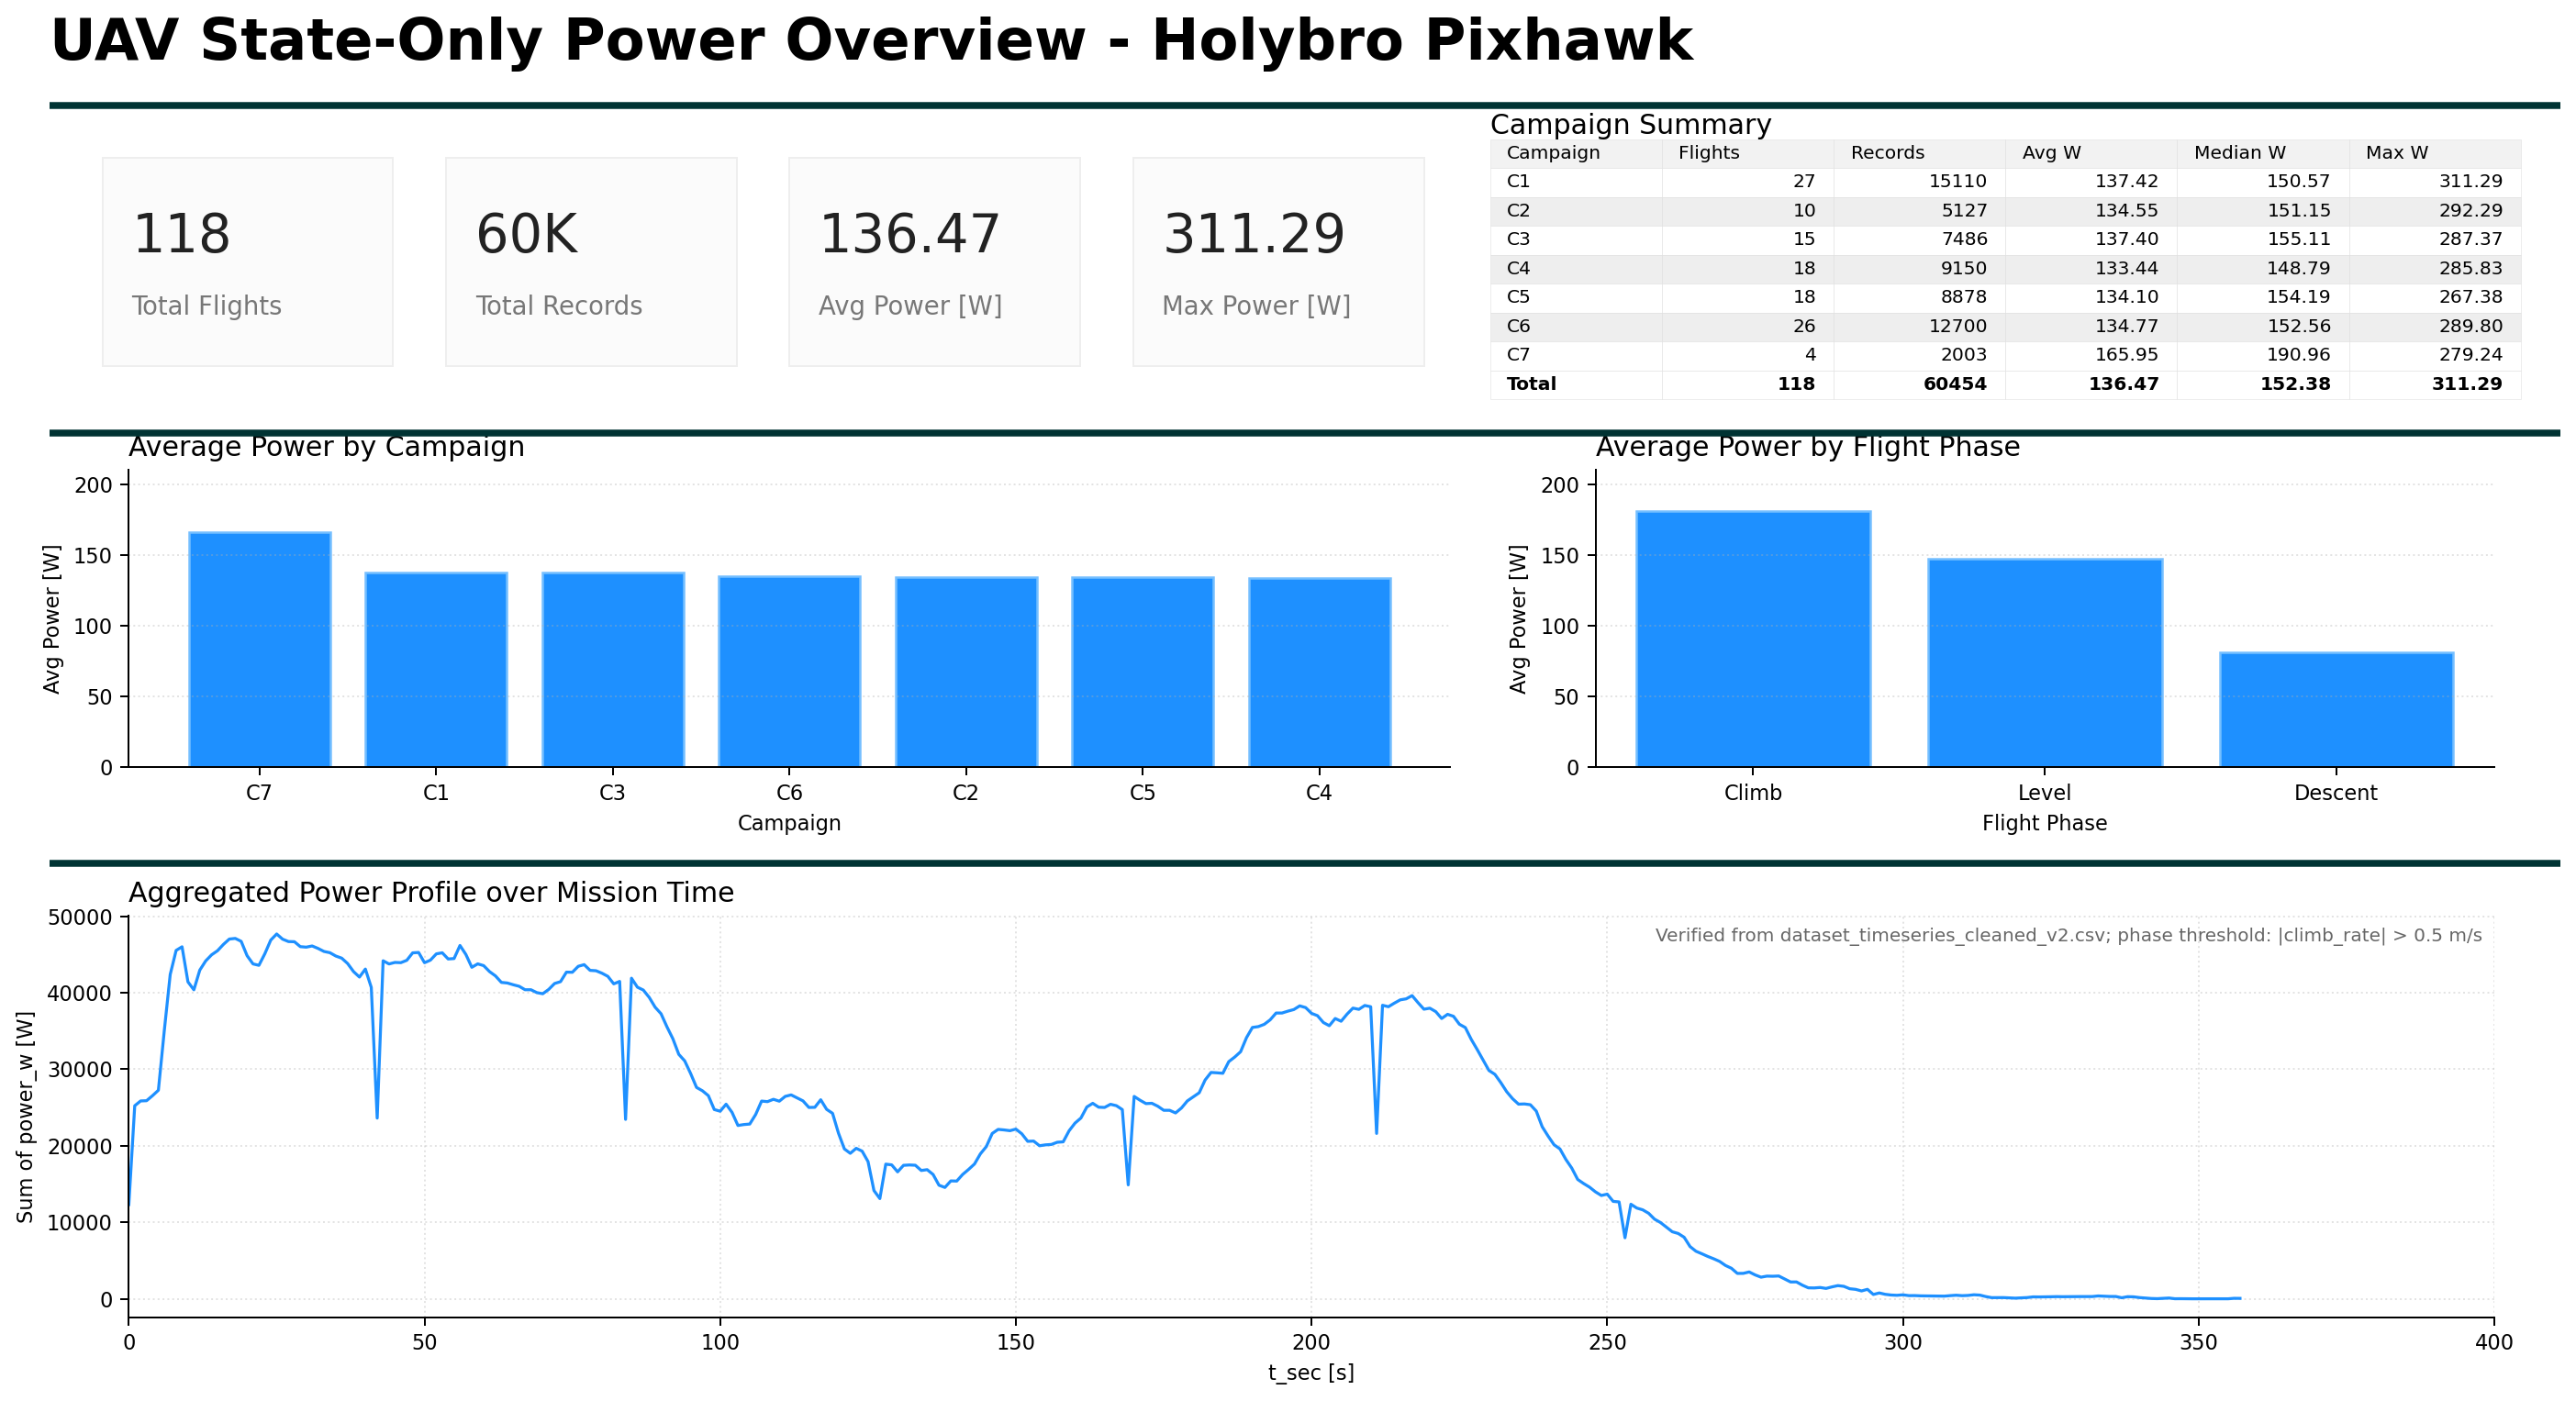
\includegraphics[width=0.92\textwidth]{target_figures/idf_state_only_overview.png}
  \caption{Cleaned IDF-DS state-only power overview for the retained Holybro/Pixhawk subset.}
  \label{fig:overview}
\end{figure}

\subsection{Refined Cleaning and Workflow}

The refined cleaning audit is based on telemetry provenance and input-side physical or statistical plausibility, not on future campaign power labels, RMSLE, Spearman rank, or audit operating scores. Flight-numbered candidates 1--120 are reduced to 118 retained flights because flights 16 and 113 are absent from the cleaned modeling table. The retained table has no missing cells, no duplicated flight--timestamp rows, no nonpositive-power rows, and no additional Stage-0 deletions, imputations, unit conversions, resampling, or row adjustments. Physical checks on speed, air density, attitude, temperature, timestamp monotonicity, and sampling intervals did not justify another removal rule.

The retained subset has mean power 136.47\,W, median power 152.38\,W, and maximum power 311.29\,W. C7 has the highest mean power, so it is treated as a late-campaign stress case rather than hidden inside the aggregate score.

\begin{figure}[!htbp]
  \centering
  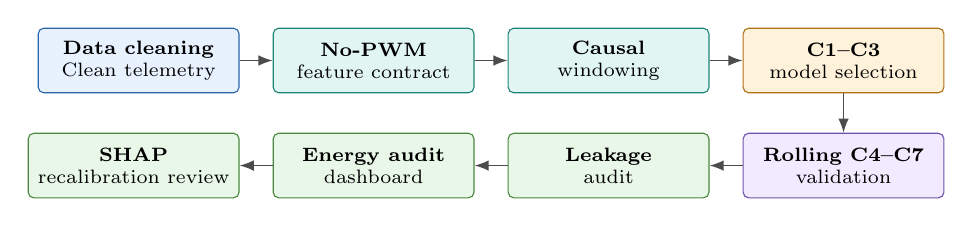
\begin{tikzpicture}[
    wfbox/.style={draw=black!65, fill=black!3, rounded corners=2pt,
      align=center, minimum width=2.55cm, minimum height=0.82cm,
      inner sep=3.5pt, font=\scriptsize},
    data/.style={wfbox, draw=wfBlueDraw, fill=wfBlueFill},
    feature/.style={wfbox, draw=wfTealDraw, fill=wfTealFill},
    model/.style={wfbox, draw=wfAmberDraw, fill=wfAmberFill},
    validation/.style={wfbox, draw=wfVioletDraw, fill=wfVioletFill},
    audit/.style={wfbox, draw=wfGreenDraw, fill=wfGreenFill},
    arrow/.style={-{Latex[length=1.8mm]}, line width=0.55pt, draw=black!70},
    node distance=0.50cm and 0.42cm
  ]
    \node[data] (clean) {\textbf{Data cleaning}\\Clean telemetry};
    \node[feature, right=of clean] (contract) {\textbf{No-PWM}\\feature contract};
    \node[feature, right=of contract] (window) {\textbf{Causal}\\windowing};
    \node[model, right=of window] (selection) {\textbf{C1--C3}\\model selection};

    \node[validation, below=of selection] (rolling) {\textbf{Rolling C4--C7}\\validation};
    \node[audit, left=of rolling] (leakage) {\textbf{Leakage}\\audit};
    \node[audit, left=of leakage] (dashboard) {\textbf{Energy audit}\\dashboard};
    \node[audit, left=of dashboard] (shap) {\textbf{SHAP}\\recalibration review};

    \draw[arrow] (clean) -- (contract);
    \draw[arrow] (contract) -- (window);
    \draw[arrow] (window) -- (selection);
    \draw[arrow] (selection) -- (rolling);
    \draw[arrow] (rolling) -- (leakage);
    \draw[arrow] (leakage) -- (dashboard);
    \draw[arrow] (dashboard) -- (shap);
  \end{tikzpicture}
  \caption{Leakage-audited No-PWM workflow from cleaning to human review.}
  \label{fig:workflow}
\end{figure}
\FloatBarrier

\subsection{State-Time Feature Policy}

The feature policy is part of the scientific claim. Allowed inputs describe vehicle motion, attitude, air data, wind context, physically interpretable derived quantities, elapsed mission time, and deterministic periodic time encodings already known at prediction time. Excluded fields include identifiers, campaign labels, the power target, target histories, motor PWM, throttle, actuator/control channels, voltage, current, battery variables, absolute route coordinates, heading, yaw, centered windows, leads, flight progress, and time-to-end. Elapsed time is observable at $t$; time-to-end is not.

\begin{table}[!htbp]
\caption{Feature inventory and leakage controls in the state-time pipeline.}
\label{tab:features}
\centering
{\small
\begin{tabular}{lcp{7.1cm}}
\toprule
Group & Count & Interpretation \\
\midrule
No-PWM candidate state-time & 40 & Leakage-screened current variables before collinearity audit \\
Shared audited state-time & 26 & Final Ridge, LSTM, TCN, and GRU input after C1--C3 Pearson/VIF pruning \\
Linear/physics auxiliaries & 1/6 & Low-dimensional references with separate VIF-safe audits \\
Causal sequence window & 64 & Past and current samples only, reset within each flight \\
Retained time features & 10 & Elapsed/log time and deterministic periodic encodings \\
\bottomrule
\end{tabular}
}
\end{table}

The multivariate Ridge, LSTM, TCN, and final GRU share the audited 26-feature state-time contract. Before multivariate auxiliary and final GRU training, deterministic and near-duplicate inputs are removed using only C1--C3, leaving no absolute Pearson pair above 0.90 and no VIF above 10 in the audited feature set; the same threshold check remains satisfied on C1--C7. A C1--C3 association audit suggests that pitch, climb behavior, airspeed, dynamic pressure, wind, and mission-time phase are plausible state-only predictors. This audit is descriptive and is not used to tune future folds.

\subsection{PWM Ablation for Feature Policy}

\begin{table}[!htbp]
\caption{Matched PWM ablation under rolling C4--C7 validation.}
\label{tab:pwmablation}
\centering
{\small
\begin{tabular}{lcccl}
\toprule
Evaluation setting & RMSE\,(W) & MAE\,(W) & RMSLE & Selected model \\
\midrule
PWM-aware ablation & 14.83 & 11.38 & 0.1566 & Log-geometric ensemble \\
No-PWM benchmark & 20.92 & 15.16 & 0.2514 & VIF-safe GRU \\
\bottomrule
\end{tabular}
}
\end{table}

The ablation in Table~\ref{tab:pwmablation} isolates the informational penalty of the No-PWM constraint under the same C4--C7 rolling test window and chronological C7 calibration boundary. Actuator commands lie on a direct pathway to electrical demand, so the PWM-aware task is easier. The No-PWM result quantifies residual uncertainty when the internal controller is treated as a black box.

\subsection{Causal Features and Model}

Derived variables are included for physical interpretability. Dynamic pressure is
\begin{equation}
  q_t = \tfrac{1}{2}\rho_t V_t^2,
  \label{eq:q}
\end{equation}
where $\rho_t$ is air density and $V_t$ is true airspeed. Positive climb and sink terms separate vertical-motion regimes, and periodic encodings avoid angular discontinuities. Transparent references show how much can be explained by simple physical cues; temporal neural references test whether ordered No-PWM context improves future-campaign power estimation. The architecture-search grid is constrained to early development campaigns C1--C3. The selected GRU is kept unchanged for C4--C7 except for the explicitly reported chronological C7 output calibration.

\subsection{Evaluation Protocol}

The outer evaluation is rolling future campaign validation:
\[
  \text{C1--C3}\to\text{C4},\quad
  \text{C1--C4}\to\text{C5},\quad
  \text{C1--C5}\to\text{C6},\quad
  \text{C1--C6}\to\text{C7}.
\]
All tuning and early stopping use only campaigns prior to the outer test campaign. The primary metric is RMSLE, the root mean squared error after applying $\log(1+P)$ to both predicted and observed power. RMSLE emphasizes relative error and reduces domination by high-power peaks. RMSE and MAE retain watt-scale interpretability, and $R^2$ measures level fit. For the selected GRU, first-difference $R^2$ is also reported as a compact check of local temporal changes~\cite{hyndman2006forecast}.

%------------------------------------------------------------------------
\section{Results}

\subsection{Baseline Behavior}

The baseline comparison establishes task difficulty. A pitch-only reference is transparent but incomplete, the physics proxy adds aerodynamic structure, Ridge tests multivariate VIF-safe state cues, and the sequence models test whether ordered No-PWM context adds useful information.

\begin{figure}[!htbp]
  \centering
  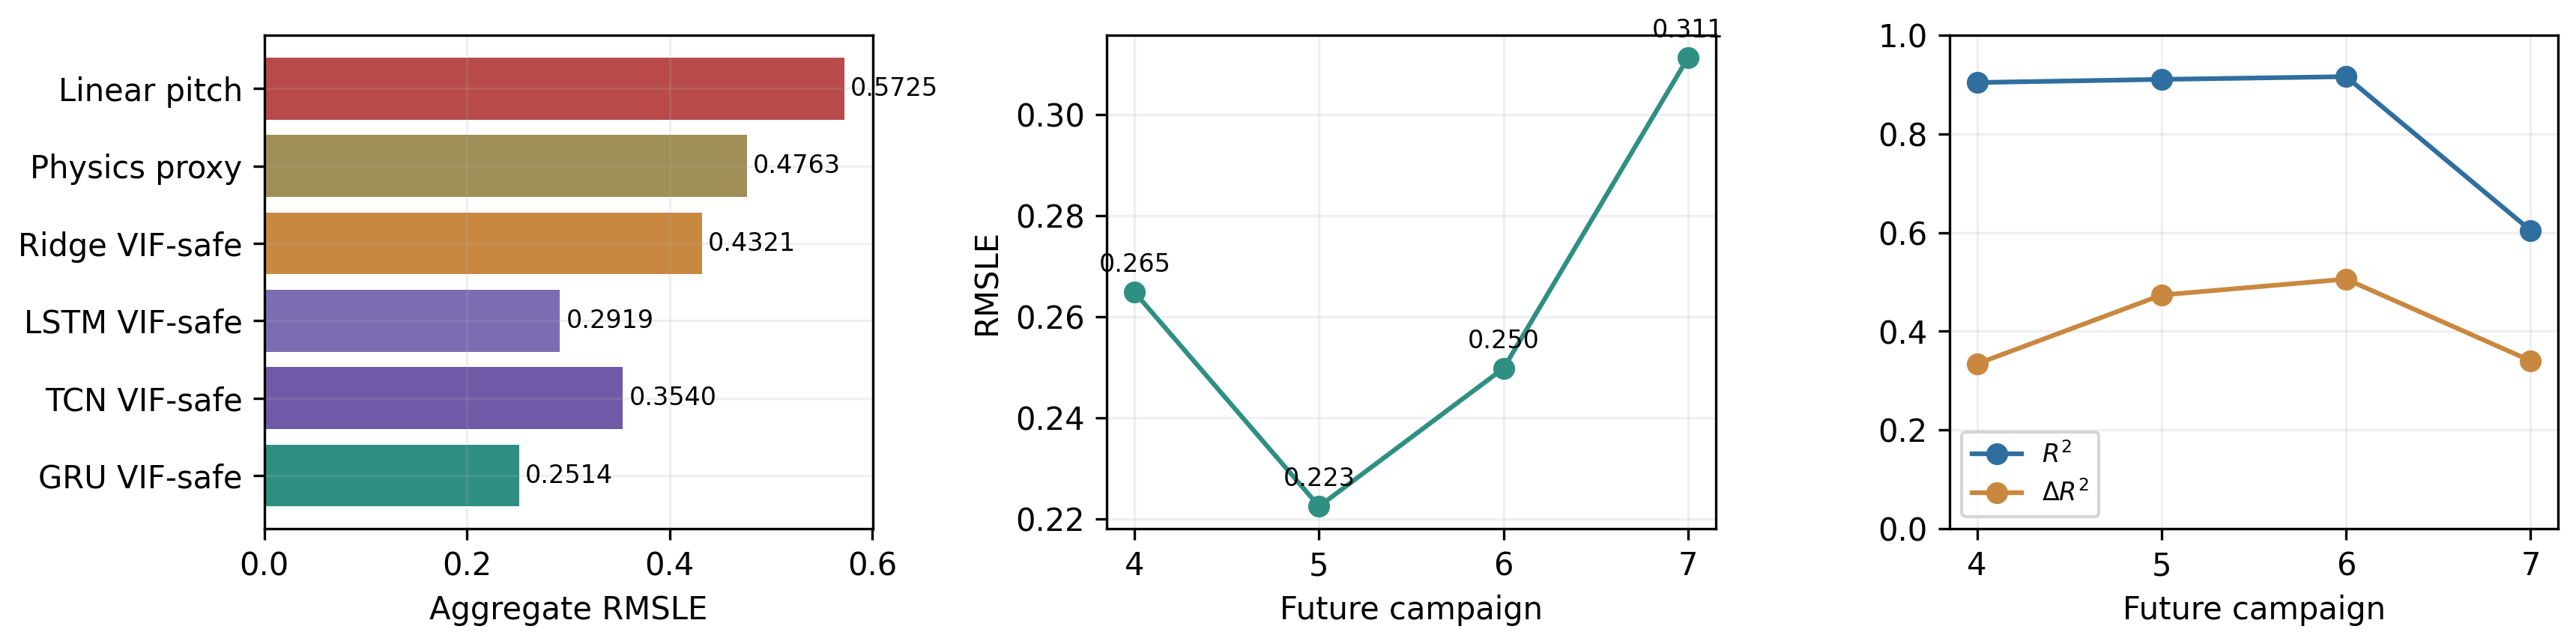
\includegraphics[width=0.95\textwidth]{target_figures/model_comparison.png}
  \caption{Aggregate RMSLE comparison and fold-level VIF-safe GRU performance.}
  \label{fig:perf}
\end{figure}
\FloatBarrier

\subsection{Future Campaign Performance}

The aggregate comparison in Table~\ref{tab:results} shows that the No-PWM task is learnable. After actuator, electrical, route-identifying, target-history, and future-derived inputs are removed, state and time history still support credible future-campaign power estimation. The selected VIF-safe GRU achieves aggregate RMSLE 0.2514, RMSE 20.92\,W, MAE 15.16\,W, and $R^2=0.8927$.

\begin{table}[!htbp]
\caption{Aggregate C4--C7 rolling future comparison under the same No-PWM feature policy.}
\label{tab:results}
\centering
{\small
\begin{tabular}{lcccc}
\toprule
Model & RMSE\,(W) & MAE\,(W) & RMSLE & $R^2$ \\
\midrule
Linear pitch & 58.85 & 45.31 & 0.5725 & 0.1507 \\
Physics proxy & 59.52 & 41.65 & 0.4763 & 0.1314 \\
Ridge VIF-safe & 45.22 & 32.93 & 0.4321 & 0.4986 \\
LSTM VIF-safe & 25.97 & 18.56 & 0.2919 & 0.8346 \\
TCN VIF-safe & 37.64 & 30.14 & 0.3540 & 0.6527 \\
GRU VIF-safe + chron. C7 cal. & \textbf{20.92} & \textbf{15.16} & \textbf{0.2514} & \textbf{0.8927} \\
\bottomrule
\end{tabular}
}
\end{table}

The physics proxy has lower watt-scale $R^2$ than the linear pitch reference even though its RMSLE is better, because RMSLE scores relative error after the log transform whereas $R^2$ scores variance explained in watt space. The transparent references show useful but incomplete energy cues, Ridge shows what a regularized current-state reference can recover after pruning, and the recurrent models show the value of ordered context.

The fold results in Table~\ref{tab:foldgru} give the main deployment lesson. C4--C6 transfer well when future campaigns remain close to the development regime, with RMSE between 18.56 and 19.42\,W. C7 exposes late-campaign distribution shift or concept drift: RMSE rises to 40.82\,W even after bounded C7 calibration. The weaker first-difference fit indicates that the model is better suited to energy demand estimation than to exact spike timing.

\begin{table}[!htbp]
\caption{Fold-level selected GRU performance on future campaigns.}
\label{tab:foldgru}
\centering
{\small
\begin{tabular}{lcccccc}
\toprule
Campaign & RMSE\,(W) & MAE\,(W) & RMSLE & RMSLE 95\% CI & $R^2$ & $\Delta R^2$ \\
\midrule
C4 & 19.42 & 14.74 & 0.2649 & [0.2391, 0.2921] & 0.9040 & 0.3342 \\
C5 & 18.85 & 14.04 & 0.2225 & [0.2114, 0.2368] & 0.9104 & 0.4735 \\
C6 & 18.56 & 14.02 & 0.2498 & [0.2287, 0.2688] & 0.9159 & 0.5057 \\
C7 & 40.82 & 29.28 & 0.3113 & [0.2094, 0.4471] & 0.6044 & 0.3403 \\
\bottomrule
\end{tabular}
}
\end{table}
\FloatBarrier

\subsection{Leakage Controls and Residual Structure}

The leakage audit contrasts the valid rolling protocol with an invalid random-row reference, which leaks similar timestamps from the same flights and campaigns across the split. Residual checks show good level tracking but heavy-tailed errors and transition mistakes. Aggregate accuracy is therefore not presented as perfect maneuver tracking, and the C7 calibration boundary remains explicit.

\subsection{Smart City Energy Audit Support}

The audit layer uses the same held-out GRU predictions for flight-level energy indicators and preliminary attribution. Its purpose is to support human review of fleet energy use, battery logs, and recalibration needs; it does not automate flight dispatch. Algorithm~\ref{alg:audit} summarizes this bounded workflow.

\begin{algorithm}[!htbp]
\caption{Rolling No-PWM flight-level energy audit.}
\label{alg:audit}
\begin{algorithmic}[1]
\REQUIRE campaigns $C_{1:7}$; No-PWM set $\mathcal{S}$; GRU family $f_\theta$
\ENSURE $\hat{P}$, $\hat{E}$, watch list $W$, and review notes $A$
\STATE Retain the cleaned, leakage-audited telemetry table.
\STATE Build 64-step causal windows from $\mathcal{S}$ within each flight.
\STATE Select the VIF-safe GRU using C1--C3 evidence only.
\FOR{$r=3,\ldots,6$}
  \STATE Train $f_\theta$ on $C_{1:r}$.
  \STATE Predict the future campaign $C_{r+1}$.
\ENDFOR
\STATE Apply the chronological C7 output-calibration boundary.
\STATE Aggregate timestamp predictions into flight energy $\hat{E}_f$.
\STATE Flag flights by the 10.1057\,Wh threshold and batch policy.
\STATE Add SHAP and recalibration notes for human review.
\RETURN $(\hat{P}, \hat{E}, W, A)$
\end{algorithmic}
\end{algorithm}

The routine starts from the cleaned telemetry table, builds causal No-PWM windows, trains the GRU under the rolling split, and converts timestamp-level predictions into flight-level energy. Its audit outputs are predicted Wh, watch-list status, error context, and SHAP/recalibration notes for human inspection.

Measured flight energy is $E_f=(1/3600)\sum_t P_{f,t}\Delta t_f$ Wh, and predicted flight energy is $\hat{E}_f=(1/3600)\sum_t\hat{P}_{f,t}\Delta t_f$ Wh, using each flight's median sampling interval. The 10.1057\,Wh watch threshold is pre-registered from the C1--C3 median before final evaluation. Flights near the threshold or under C7-like shift warnings are routed to battery-log inspection and recalibration review. The batch-limited top-nine queue reaches 66.7\% precision and 66.7\% recall for high-energy flight review while limiting workload.

\begin{figure}[!htbp]
  \centering
  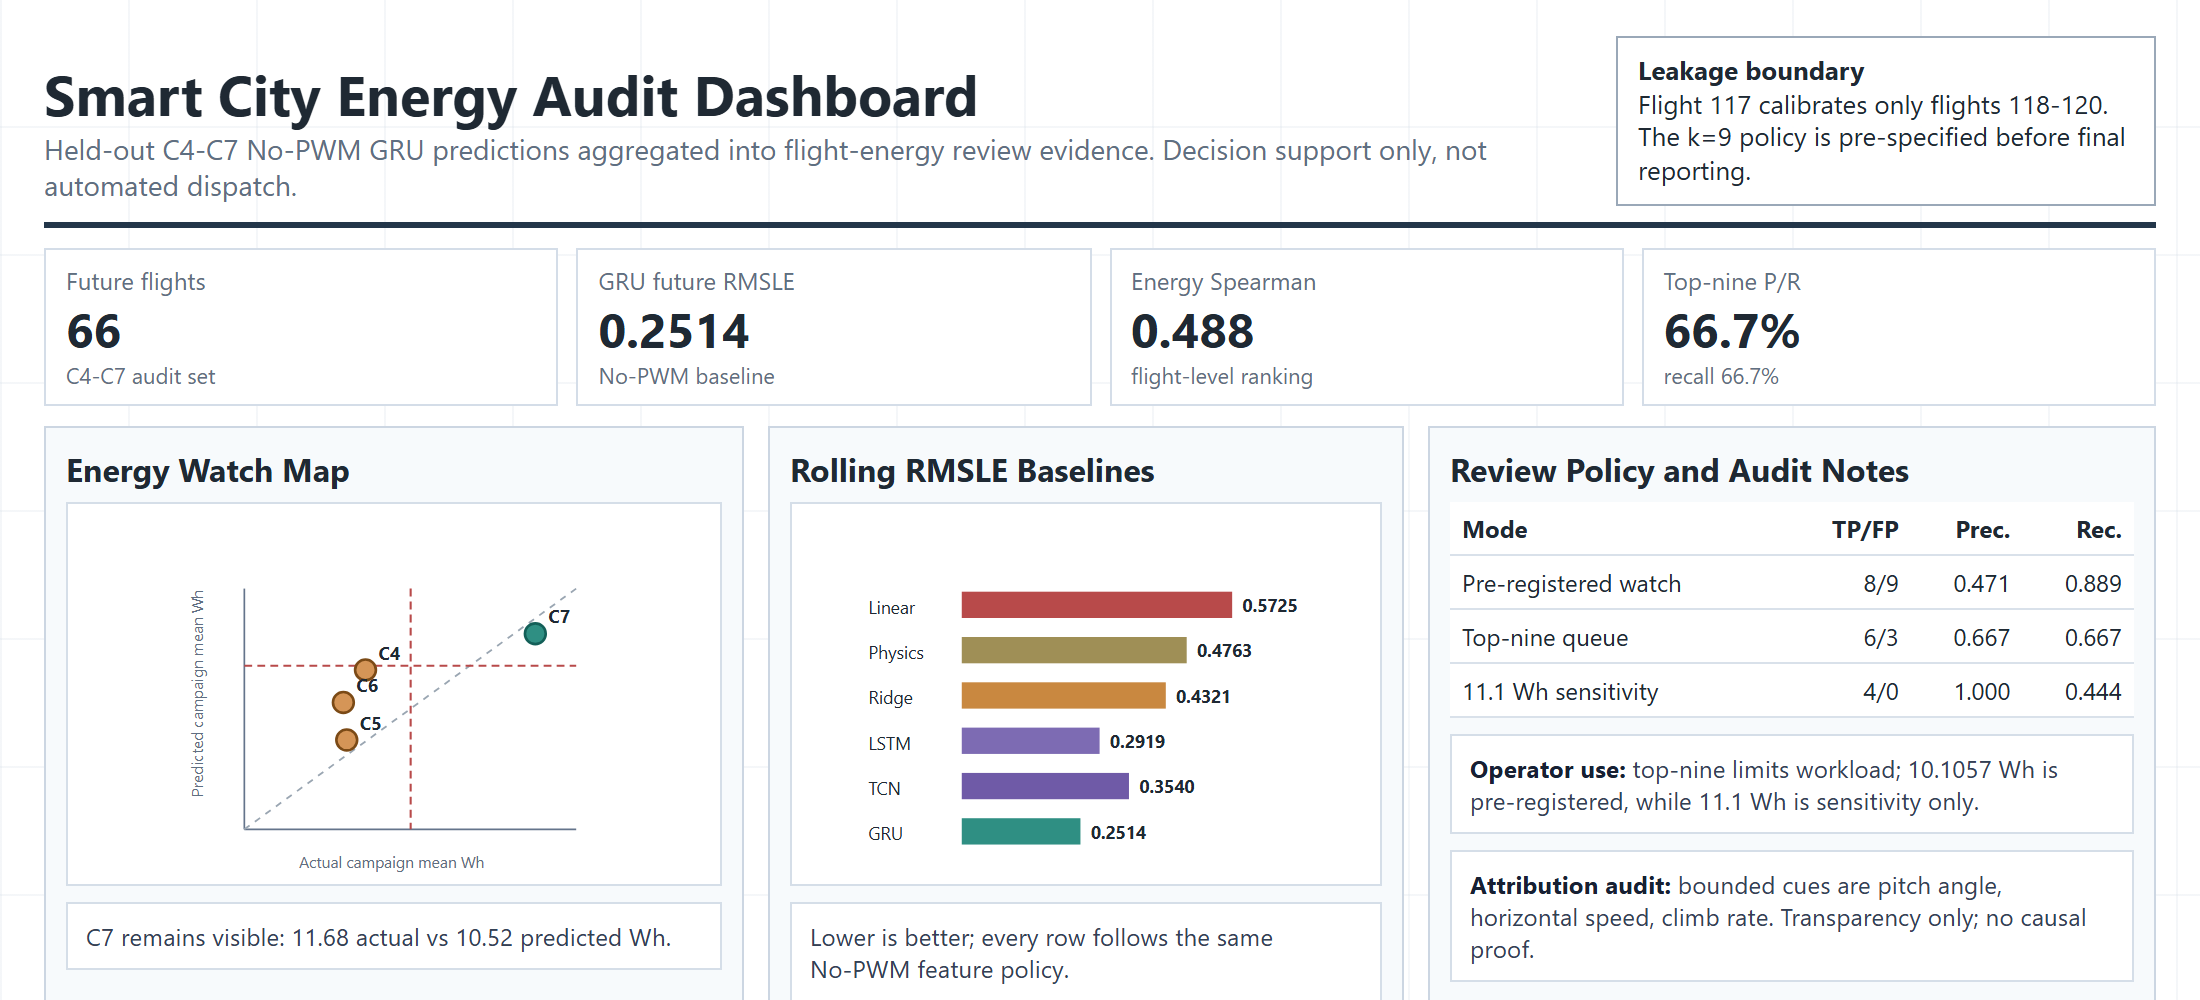
\includegraphics[width=0.95\textwidth]{target_figures/audit_dashboard.png}
  \caption{Human-reviewed Smart City energy audit dashboard from held-out predictions.}
  \label{fig:audit}
\end{figure}

The dashboard in Fig.~\ref{fig:audit} consolidates the three policy modes used for review: the pre-registered early-campaign median threshold, the batch-limited top-nine queue, and the 11.1\,Wh sensitivity point. The C7 adjustment uses no future labels for fitting. Flight 117 is the sole labeled C7 calibration flight; the fitted log-affine correction is applied only to later source IDs 118--120. These later IDs are inspected as a directional adaptation check, while the fold-level results in Table~\ref{tab:foldgru} report the full C7 fold.

The SHAP audit in Fig.~\ref{fig:shap} adds bounded attribution evidence from GradientExplainer on held-out C4--C7 windows. The strongest groups are pitch, horizontal speed, climb rate, elapsed time, and dynamic pressure. The campaign panel shows why the audit remains cautious: C7 changes the attribution pattern relative to earlier campaigns. The temporal panel places most attribution mass near the prediction time, supporting recent state history rather than future-derived information.

\begin{figure}[!htbp]
  \centering
  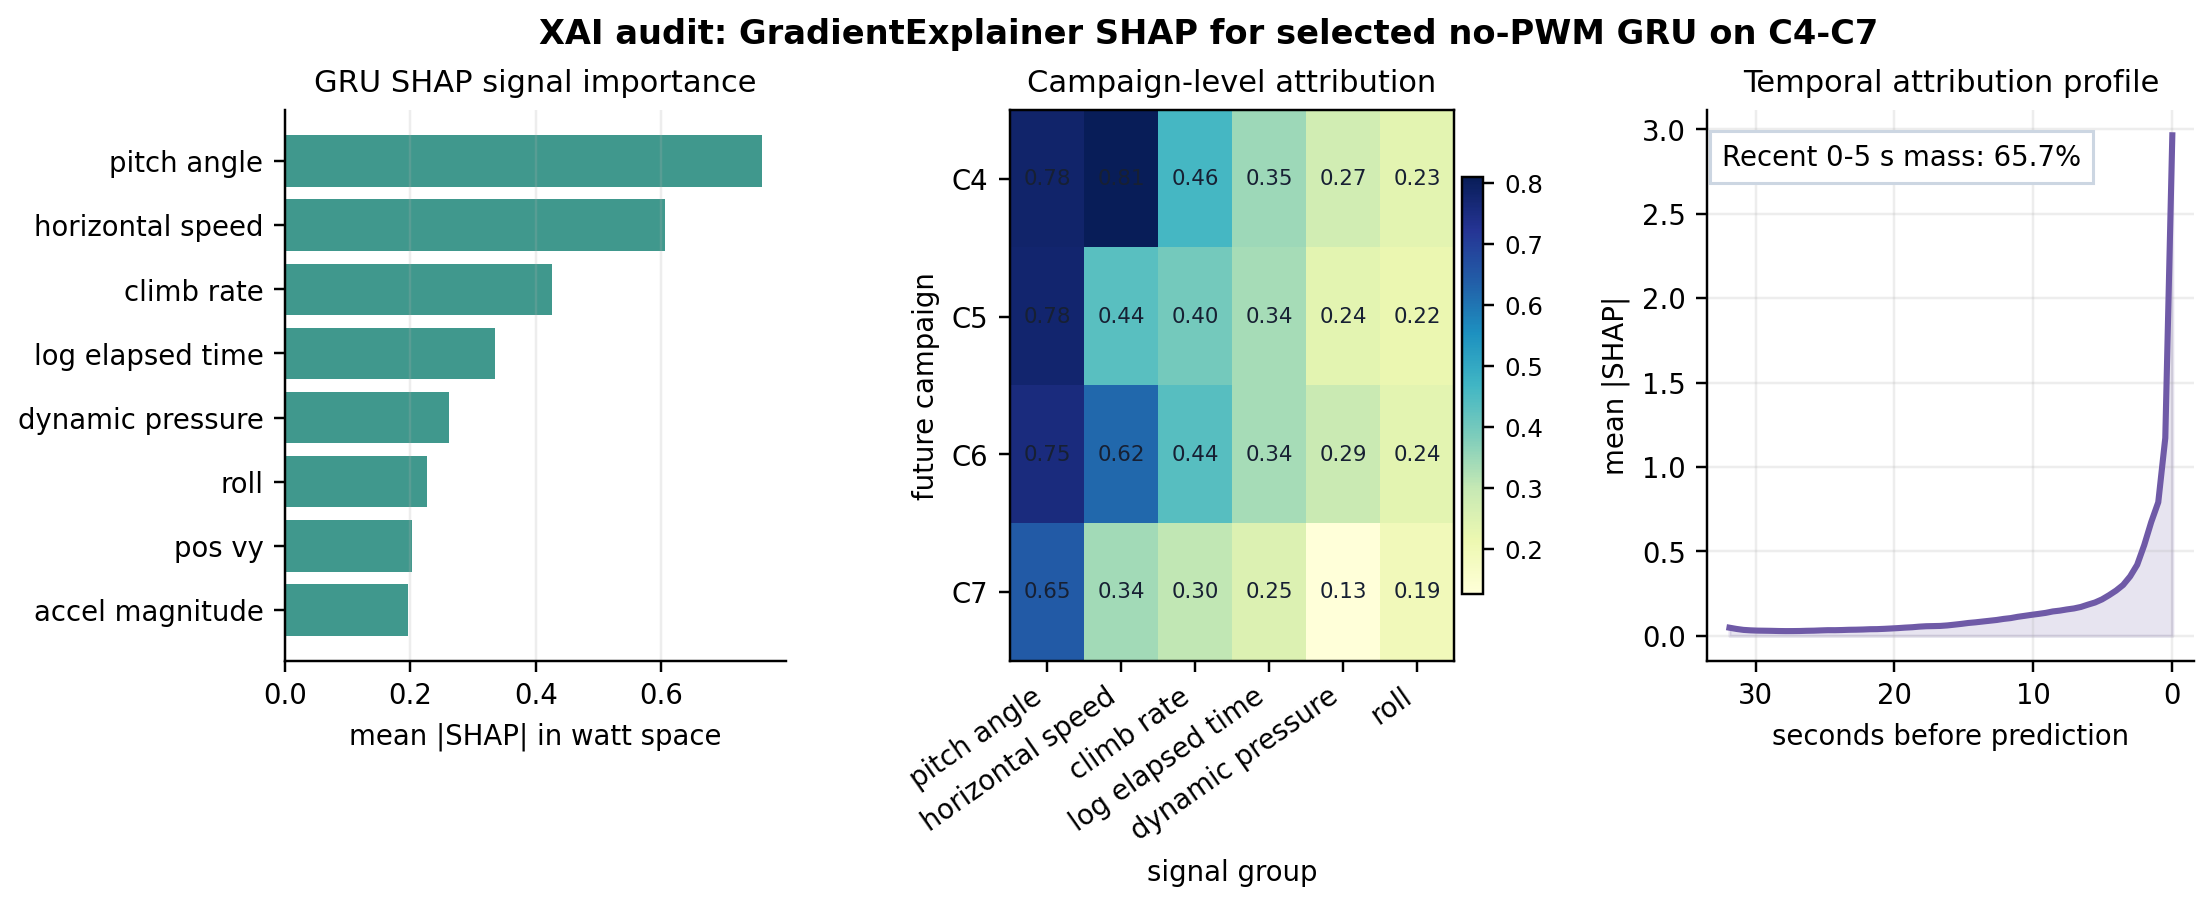
\includegraphics[width=0.98\textwidth]{target_figures/audit_shap.png}
  \caption{Bounded attribution audit for the selected No-PWM GRU on C4--C7.}
  \label{fig:shap}
\end{figure}

These explanations are model-audit evidence for human review. They make the energy dashboard more transparent, but they do not prove causality or authorize automated dispatch.
\FloatBarrier

%------------------------------------------------------------------------
\section{Discussion}

The VIF-safe GRU is credible under C4--C6, where future campaigns preserve flight dynamics and environmental conditions close to the development regime. This supports the No-PWM setting when actuator or electrical signals are unavailable, heterogeneous across platforms, or too leakage-prone for a conservative benchmark. The PWM ablation also shows why those excluded signals remain informative: the No-PWM task is intentionally harder.

C7 marks the generalization boundary. The fold RMSE of 40.82\,W and RMSLE 0.3113 indicate late-campaign distribution shift or concept drift rather than a solved deployment problem. The calibration boundary is therefore reported openly: flight 117 anchors the chronological C7 adjustment, later C7 flights are inspected after that boundary, and retrospective leave-one-flight-out grids remain diagnostic only.

The Smart City interpretation is intentionally bounded. The top-nine queue, the 10.1057\,Wh pre-registered threshold, and the 11.1\,Wh sensitivity point can guide battery-log inspection, charging-buffer review, and recalibration. They do not make dispatch decisions. A minimum field-use guard is to flag flights with suspicious shift indicators or predicted energy within the 1.2964\,Wh error band around the pre-registered watch threshold.

Remaining limitations include a single platform subset, missing payload information, unobserved battery health, controller-mode changes, gust conditions, and limited shift coverage. SHAP is used only as attribution evidence for model review; it does not establish causality. Future work should add legitimate weather metadata, improve calibrated uncertainty, run cross-platform validation, evaluate online or few-shot recalibration, and test field deployment procedures under human oversight.

%------------------------------------------------------------------------
\section{Conclusion}

Reliable UAV energy estimation is useful only when the evaluation protocol reflects future deployment conditions. This study shows that a leakage-audited No-PWM GRU can provide a credible state-time baseline on the IDF-DS telemetry subset under chronological rolling validation.

The selected VIF-safe GRU achieved aggregate RMSLE 0.2514, RMSE 20.92\,W, MAE 15.16\,W, and $R^2=0.8927$, indicating that state-time telemetry can support power estimation even without actuator and electrical inputs. The scientific value is a reproducible No-PWM feature contract, development-only multicollinearity pruning, chronological rolling validation, and a public baseline for timestamp-level power prediction.

The practical value remains deliberately bounded. The model outputs are converted into flight-level energy indicators, watch-list evidence, and recalibration cues for human-supervised UAV fleet management, not automatic dispatch or deployed city-scale control. C7 degradation highlights the need for shift-aware validation before operational use. Future work should extend the benchmark with legitimate weather metadata, calibrated uncertainty, cross-platform testing, online adaptation, and field deployment validation without reintroducing leakage.

\paragraph{Acknowledgements.}
The authors thank the IDF-DS dataset creators for releasing the fixed-wing UAS telemetry benchmark used in this study. AI-assisted tools were used only for language polishing and formatting checks; all scientific claims, experimental design, code execution, data analysis, results, and conclusions were verified by the authors.

\paragraph{Declarations.}
Funding: The authors received no specific funding. Competing interests: The authors declare no competing interests. Ethics approval and consent to participate: Not applicable. Consent for publication: Not applicable. Data and code availability: The source IDF-DS dataset is publicly available through Zenodo. The derived cleaned modeling table and notebooks are retained with the manuscript workspace and will be archived in a public repository after a stable release is prepared. Author contributions: N. Truong led the experiments and manuscript drafting. Thu Le supervised research validation. H.D. Tai contributed to experimental review.

%------------------------------------------------------------------------
\begin{thebibliography}{99}

\bibitem{shakhatreh2019survey}
Shakhatreh, H., et al.: Unmanned aerial vehicles (UAVs): A survey on civil applications and key research challenges. \textit{IEEE Access} \textbf{7}, 48572--48634 (2019). \href{https://arxiv.org/abs/1805.00881}{arXiv:1805.00881}

\bibitem{mozaffari2019tutorial}
Mozaffari, M., et al.: UAVs for wireless networks: Applications, challenges, and open problems. \textit{IEEE Communications Surveys \& Tutorials} \textbf{21}(3), 2334--2360 (2019). \href{https://arxiv.org/abs/1803.00680}{arXiv:1803.00680}

\bibitem{hayat2016survey}
Hayat, S., Yanmaz, E., Muzaffar, R.: Survey on unmanned aerial vehicle networks for civil applications: A communications viewpoint. \textit{IEEE Communications Surveys \& Tutorials} \textbf{18}(4), 2624--2661 (2016)

\bibitem{zeng2017energy}
Zeng, Y., Zhang, R.: Energy-efficient UAV communication with trajectory optimization. \textit{IEEE Transactions on Wireless Communications} \textbf{16}(6), 3747--3760 (2017). \href{https://arxiv.org/abs/1608.01828}{arXiv:1608.01828}

\bibitem{difranco2016coverage}
Di Franco, C., Buttazzo, G.: Coverage path planning for UAVs photogrammetry with energy and resolution constraints. \textit{Journal of Intelligent \& Robotic Systems} \textbf{83}, 445--462 (2016). \href{https://doi.org/10.1007/s10846-016-0348-x}{doi:10.1007/s10846-016-0348-x}

\bibitem{abeywickrama2018access}
Abeywickrama, H.V., et al.: Comprehensive energy consumption model for unmanned aerial vehicles, based on empirical studies of battery performance. \textit{IEEE Access} \textbf{6}, 58383--58394 (2018)

\bibitem{stolaroff2018drone}
Stolaroff, J.K., et al.: Energy use and life cycle greenhouse gas emissions of drones for commercial package delivery. \textit{Nature Communications} \textbf{9}, 409 (2018). \href{https://doi.org/10.1038/s41467-017-02411-5}{doi:10.1038/s41467-017-02411-5}

\bibitem{gora2022ml}
G\'ora, K., et al.: Machine Learning in creating energy consumption model for UAV. \textit{Energies} \textbf{15}(18), 6810 (2022). \href{https://doi.org/10.3390/en15186810}{doi:10.3390/en15186810}

\bibitem{zhang2021models}
Zhang, J., et al.: Energy consumption models for delivery drones: A comparison and assessment. \textit{Transportation Research Part D} \textbf{90}, 102668 (2021). \href{https://doi.org/10.1016/j.trd.2020.102668}{doi:10.1016/j.trd.2020.102668}

\bibitem{garcia2025zenodo}
Garc\'ia Gasc\'on, C.: Fixed-Wing UAS Telemetry Benchmark (IDF-DS): 240 Flights for ML and Intelligent Trajectory Optimization. Zenodo (2025). \href{https://doi.org/10.5281/zenodo.16992976}{doi:10.5281/zenodo.16992976}

\bibitem{garcia2026idfds}
Garc\'ia-Gasc\'on, C., et al.: Open benchmark data for ML and intelligent trajectory optimization in fixed-wing UAS. \textit{Scientific Data} \textbf{13}, 364 (2026). \href{https://doi.org/10.1038/s41597-026-06716-3}{doi:10.1038/s41597-026-06716-3}

\bibitem{cho2014gru}
Cho, K., et al.: Learning phrase representations using RNN encoder--decoder for statistical machine translation. In: \textit{Proceedings of the 2014 Conference on Empirical Methods in Natural Language Processing}, pp.~1724--1734. Association for Computational Linguistics (2014). \href{https://doi.org/10.3115/v1/D14-1179}{doi:10.3115/v1/D14-1179}

\bibitem{hochreiter1997lstm}
Hochreiter, S., Schmidhuber, J.: Long short-term memory. \textit{Neural Computation} \textbf{9}(8), 1735--1780 (1997). \href{https://doi.org/10.1162/neco.1997.9.8.1735}{doi:10.1162/neco.1997.9.8.1735}

\bibitem{bai2018tcn}
Bai, S., Kolter, J.Z., Koltun, V.: An empirical evaluation of generic convolutional and recurrent networks for sequence modeling. \textit{arXiv preprint} arXiv:1803.01271 (2018)

\bibitem{bergmeir2018cv}
Bergmeir, C., Hyndman, R.J., Koo, B.: A note on the validity of cross-validation for evaluating autoregressive time series prediction. \textit{Computational Statistics \& Data Analysis} \textbf{120}, 70--83 (2018). \href{https://doi.org/10.1016/j.csda.2017.11.003}{doi:10.1016/j.csda.2017.11.003}

\bibitem{kaufman2012leakage}
Kaufman, S., Rosset, S., Perlich, C., Stitelman, O.: Leakage in data mining: Formulation, detection, and avoidance. \textit{ACM Transactions on Knowledge Discovery from Data} \textbf{6}(4), Article 15 (2012). \href{https://doi.org/10.1145/2382577.2382579}{doi:10.1145/2382577.2382579}

\bibitem{lundberg2017shap}
Lundberg, S.M., Lee, S.-I.: A unified approach to interpreting model predictions. In: \textit{Advances in Neural Information Processing Systems} 30, pp.~4765--4774 (2017)

\bibitem{arrieta2020xai}
Arrieta, A.B., et al.: Explainable artificial intelligence (XAI): Concepts, taxonomies, opportunities and challenges toward responsible AI. \textit{Information Fusion} \textbf{58}, 82--115 (2020). \href{https://doi.org/10.1016/j.inffus.2019.12.012}{doi:10.1016/j.inffus.2019.12.012}

\bibitem{batty2012smart}
Batty, M., et al.: Smart cities of the future. \textit{European Physical Journal Special Topics} \textbf{214}, 481--518 (2012). \href{https://doi.org/10.1140/epjst/e2012-01703-3}{doi:10.1140/epjst/e2012-01703-3}

\bibitem{hyndman2006forecast}
Hyndman, R.J., Koehler, A.B.: Another look at measures of forecast accuracy. \textit{International Journal of Forecasting} \textbf{22}(4), 679--688 (2006). \href{https://doi.org/10.1016/j.ijforecast.2006.03.001}{doi:10.1016/j.ijforecast.2006.03.001}

\end{thebibliography}

\end{document}
